\documentclass[journal=jcisd8,manuscript=article]{achemso}

\setkeys{acs}{articletitle=true,doi=true}

\usepackage[utf8]{inputenc}
\usepackage[T1]{fontenc}
\usepackage{amsmath,amssymb}
\usepackage{booktabs}
\usepackage{graphicx}
\usepackage{array}
\usepackage{url}
\usepackage{xcolor}

\author{Changtian Qian}
\email{qianchangdtw@gmail.com}
\affiliation[Capital Normal University]{Department of Physics, Capital Normal University, Beijing 100048, China}

\title[QuantumChem AI]{QuantumChem AI: A Rule-Governed Automation Platform with Grounded LLM Assistance for All-Element Atomic Cluster Quantum Chemistry}

\keywords{atomic clusters, quantum chemistry automation, density functional theory, Design Constitution, LLM hallucination guard, isomer deduplication, lanthanide superatoms}

\begin{document}
\sloppy

\begin{abstract}
Automated quantum-chemical workflows for atomic clusters across the periodic table must coordinate global configurational search, rotation- and permutation-invariant isomer deduplication, basis-set and effective core potential (ECP) matching, open-shell spin-multiplicity scanning, fault-tolerant high-performance computing (HPC) orchestration, wavefunction post-processing, and publication-grade visualization. Conventional workflows typically hardcode specific element families, omit systematic spin-state and wavefunction stability verification, or expose large language model (LLM) assistants to unverified numerical hallucinations. This work presents QuantumChem AI, an open-source automation platform built upon a reuse-first architecture and an eight-article Design Constitution (C1--C8) enforced across runtime validators and continuous integration. First, a periodic-table-general YAML rule engine---verified by Python abstract syntax tree (AST) static analysis to contain zero element-symbol conditional branches---integrates Basis Set Exchange (\texttt{GenECP}) coverage verification, electron-parity conservation, Hund-rule atomic multiplicities, and adaptive spin-multiplicity scanning with early stopping and boundary expansion. Second, a three-stage geometric deduplicator combines distance-matrix eigenvalue fingerprinting with tri-axial principal-inertia Hungarian/Kabsch alignment to reach $10^{-15}$~\AA\ equivalence precision in under 8~ms, paired with point-group symmetry dopant enumeration. Third, a shared-HPC scheduler performs NUMA topology probing, user-load throttling, elastic core scaling (4 to 10--16 cores), SSH auto-reconnect with exit-poll race protection, three-section \texttt{--Link1--} (\texttt{opt} $\rightarrow$ \texttt{stable=opt} $\rightarrow$ \texttt{freq}) decomposition, and lossless $4f$ self-consistent field (SCF) and input-tail recovery. Fourth, deterministic physical-property analysis couples version-locked Multiwfn 3.8(dev) parsing with dual-engine Matplotlib/Origin 2024b plotting, inertia-aligned VMD/py3Dmol 3D rendering, and A4 PDF report compilation. Fifth, a \texttt{pydantic-ai} natural-language planning and read-only interpretation layer enforces deterministic \texttt{build\_plan()} validation and unit-conversion-aware numerical grounding, achieving 50/50 (100.0\%) accuracy across both Chinese and matched English scientific instruction benchmarks on \texttt{deepseek-v4.1-flash}. Validation across 10 reference Gaussian 16 cluster benchmarks, Multiwfn analysis of $\mathrm{Al_{12}Cu}$, and an autonomous 9-project, 230-job (221 Gaussian 16 runs, 1,399.78 CPU core-hours, 100\% convergence with 7 automated $4f$ repairs) study of heavy lanthanide $\mathrm{Ln@Au_5}$ ($\mathrm{Ln} = \mathrm{Gd\text{--}Lu}$) identifies a trivalent $8\mathrm{e}^-$ superatom HOMO--LUMO gap rigidity plateau (2.524--2.812~eV), localized $4f$ spin decoupling, and a divalent $\mathrm{Yb^{2+}}$ ($4f^{14}$, $7\mathrm{e}^-$) gap collapse and spin delocalization transition.
\end{abstract}

\section{Introduction}

Atomic clusters bridge isolated atoms and extended condensed-matter phases, exhibiting pronounced size-dependent shell closures, superatom electronic stability, tunable magnetic moments, and site-selective catalytic activity.\cite{pyykko2002wau12,li2002wau12,jian2019pes} Conducting rigorous density functional theory (DFT) investigations across diverse cluster chemistries requires orchestrating heterogeneous software ecosystems: global potential-energy-surface exploration (e.g., ABCluster\cite{zhang2015abcluster} or tight-binding genetic algorithms\cite{bannwarth2019gfn2xtb,larsen2017ase}), geometric isomer deduplication, consistent basis-set and relativistic effective core potential (ECP) assignment,\cite{weigend2005def2,pritchard2019bse,dolg2012ecp} open-shell spin-state scanning,\cite{cramer2009tm} fault recovery on shared Linux servers,\cite{ong2013pymatgen} wavefunction analysis,\cite{oboyle2008cclib,lu2012multiwfn} and publication-ready figure generation.\cite{humphrey1996vmd}

Although mature individual libraries excel at isolated stages, four critical methodological and engineering barriers hinder reliable end-to-end cluster discovery across the full periodic table (Table~\ref{tab:capabilities}):
\begin{enumerate}
  \item \textbf{Element-specific fragmentation:} In-house workflows frequently hardcode DFT functionals, basis sets, and trial multiplicities for narrow chemical families (such as pure gold or silicon clusters), failing or producing inconsistent physics when transferred to open-shell $3d$/$5d$ transition metals, bimetallic alloys, or $4f$ lanthanide-doped clusters.
  \item \textbf{Silent physical inconsistencies:} Without automated enforcement of identical levels of theory across clusters and atomic references, systematic $\langle S^2 \rangle$ spin-contamination auditing, and \texttt{stable=opt} wavefunction stability verification,\cite{bauernschmitt1996stability} computed binding energies, stabilities, and magnetic moments remain vulnerable to hidden artifacts.
  \item \textbf{Fragile shared-HPC orchestration:} Academic cluster servers often operate without centralized job schedulers such as Slurm or PBS and host concurrent multi-user workloads. Naive parallel submission causes NUMA cross-socket contention and resource exhaustion, while Gaussian SCF convergence failures (\texttt{L502}), optimization step limits (\texttt{L9999}), and saddle-point imaginary modes require automated server-side recovery.
  \item \textbf{LLM numerical hallucinations:} Directly querying general-purpose large language models (LLMs) over quantum-chemical logs invites fabricated energies, gaps, and structural parameters, even in tool-augmented scientific agents.\cite{bran2024chemcrow,boiko2023coscientist}
\end{enumerate}

\begin{table}[htbp]
  \centering
  \caption{Core Capabilities of QuantumChem AI Compared with Conventional Cluster Scripts and General High-Throughput Material Frameworks}
  \label{tab:capabilities}
  \footnotesize
  \begin{tabular}{>{\raggedright\arraybackslash}p{2.4cm} >{\raggedright\arraybackslash}p{3.6cm} >{\raggedright\arraybackslash}p{3.7cm} >{\raggedright\arraybackslash}p{4.3cm}}
    \toprule
    Capability Dimension & Conventional Manual Scripts & General High-Throughput Frameworks & QuantumChem AI (This Work) \\
    \midrule
    Elemental scope & Hardcoded to narrow chemical families & Focused on periodic crystals and bulk solids & Full periodic table (H--Rn \& lanthanides); AST-enforced zero element branches \\
    Spin \& stability rigor & Manual trial multiplicities; \texttt{stable=opt} often omitted & Periodic spin polarization; molecular \texttt{--Link1--} rare & Parity conservation + adaptive early-stop/expansion + 3-section \texttt{--Link1--} loop \\
    Shared-HPC scheduling & Manual \texttt{nohup}/\texttt{screen}; prone to node overload & Dependent on Slurm/PBS queue managers & Scheduler-free \texttt{ShellIO} + NUMA probing + load throttling + elastic core scaling \\
    Analysis \& visualization & Manual Excel/Origin/VMD switching & Matplotlib previews; sparse Origin/VMD integration & Multiwfn 3.8(dev) version lock + 10 dual-engine plot types + VMD ray tracing + A4 PDF \\
    LLM collaboration & Absent or ungrounded chat & Minimal validated planning/analysis coupling & \texttt{pydantic-ai} NL planner + unit-aware numerical anti-hallucination guard \\
    \bottomrule
  \end{tabular}
\end{table}

To unify deterministic physical rigor with natural-language accessibility, this work introduces QuantumChem AI. Guided by a reuse-first software architecture over established scientific libraries (ASE,\cite{larsen2017ase} pymatgen/custodian,\cite{ong2013pymatgen} Basis Set Exchange,\cite{pritchard2019bse} cclib,\cite{oboyle2008cclib} and Multiwfn\cite{lu2012multiwfn}), the platform embeds an eight-article Design Constitution directly into its runtime validators and test suite, creating a verifiable closed loop from natural language to superatom discovery and publication deliverables.

\section{System Architecture and Design Constitution}

\subsection{Eight-Article Design Constitution (C1--C8)}

Inspired by explicit rule-based governance,\cite{bai2022constitutional} QuantumChem AI enforces an eight-article Design Constitution (C1--C8) at both continuous-integration (CI) and runtime execution boundaries:
\begin{itemize}
  \item \textbf{C1 (Numerical Determinism):} All energies, relative stabilities, HOMO--LUMO gaps, binding energies, spin expectation values, and charge/spin populations are computed exclusively by deterministic Python, cclib, and Multiwfn pipelines and persisted to structured storage. LLMs never estimate or fabricate physical quantities; every natural-language interpretation must pass a deterministic numerical grounding guard.
  \item \textbf{C2 (Zero Element-Symbol Hardcoding):} Conditional branches referencing explicit chemical symbols (e.g., \texttt{if symbol == "Au"}) are strictly prohibited throughout \texttt{src/}. All rules query intrinsic periodic-table attributes (atomic number $Z$, group, period, block $s/p/d/f$, valence shell occupancy). An automated AST scanner (\texttt{test\_axiom\_no\_\allowbreak{}element\_branches.py}) audits every source module on every test run.
  \item \textbf{C3 (Single-Source Rules \& Decision Provenance):} Theory tiers, dispersion corrections, multiplicity bounds, charge templates, and research recipes reside solely in \texttt{src/qcai/knowledge/rules/*.yaml} alongside physical rationales and literature citations. Every generated \texttt{Decision} records its rule identifier and human-override status.
  \item \textbf{C4 (Theory-Level Consistency):} Comparative energetic observables---binding energy ($E_b$), second energy difference ($\Delta_2 E$), fragmentation energy ($E_f$), embedding energy ($E_{\text{emb}}$), substitution energy ($E_{\text{sub}}$), mixing excess energy ($\Delta$), and vertical/adiabatic electron detachment energies (VDE/ADE)---enforce identical functionals, dispersion corrections, basis sets, and ECP definitions across clusters, isolated atoms, and ionic references.
  \item \textbf{C5 (Data--Rendering Decoupling):} The analysis layer emits tool-agnostic \texttt{FigureSpec} objects consumed independently by \texttt{MatplotlibRenderer} and \texttt{OriginRenderer}, guaranteeing identical underlying physics across offline previews and editable OriginLab \texttt{.opju} publication graphics.
  \item \textbf{C6 (Credential Isolation \& Zero Echo):} SSH host keys, private file paths, and LLM API keys never enter version control, runtime logs, diagnostic bundles, or LLM prompt contexts. API credentials reside in the operating-system keyring.
  \item \textbf{C7 (Shared-Cluster Courtesy \& Idempotent Recovery):} All pipeline stages persist to SQLite with pause/resume reconciliation across restarts. Live server probing suspends new submissions when competing users saturate host compute resources.
  \item \textbf{C8 (Automatic Defect Surfacing):} Imaginary frequencies, wavefunction instabilities, $\langle S^2 \rangle$ spin contamination, custodian recovery histories, and $4f$ multi-reference advisories aggregate automatically into \texttt{ProjectSummary.all\_issues} and propagate explicitly to the web workbench, PDF reports, and AI summaries.
\end{itemize}

\subsection{Five-Layer Stack and S0--S7 Multi-Fidelity Funnel}

As illustrated in Figure~\ref{fig:arch}a, QuantumChem AI decouples responsibilities across five deterministic layers connected by strict Pydantic data contracts (\texttt{ResearchRequest}, \texttt{CalcPlan}, \texttt{JobSpec}, and \texttt{CalcResult}), while six generic plugin registries (\texttt{Registry[T]}) govern extensible backends: \texttt{QCPROGRAMS} (Gaussian 16,\cite{frisch2019g16} extensible to ORCA/CP2K), \texttt{GENERATORS} (structure import, ABCluster, Molclus, ASE-GA), \texttt{RENDERERS} (Matplotlib, Origin 2024b), \texttt{RUNNERS} (SSH \texttt{DirectRunner}, \texttt{MockRunner}), \texttt{LLMS} (\texttt{DeepSeekLLMProvider}), and \texttt{PROFILES} (\texttt{ClusterProfile}). Figure~\ref{fig:arch}b details the constitutional closed-loop LLM controllers governing natural-language planning and result interpretation.

\begin{figure}[htbp]
  \centering
  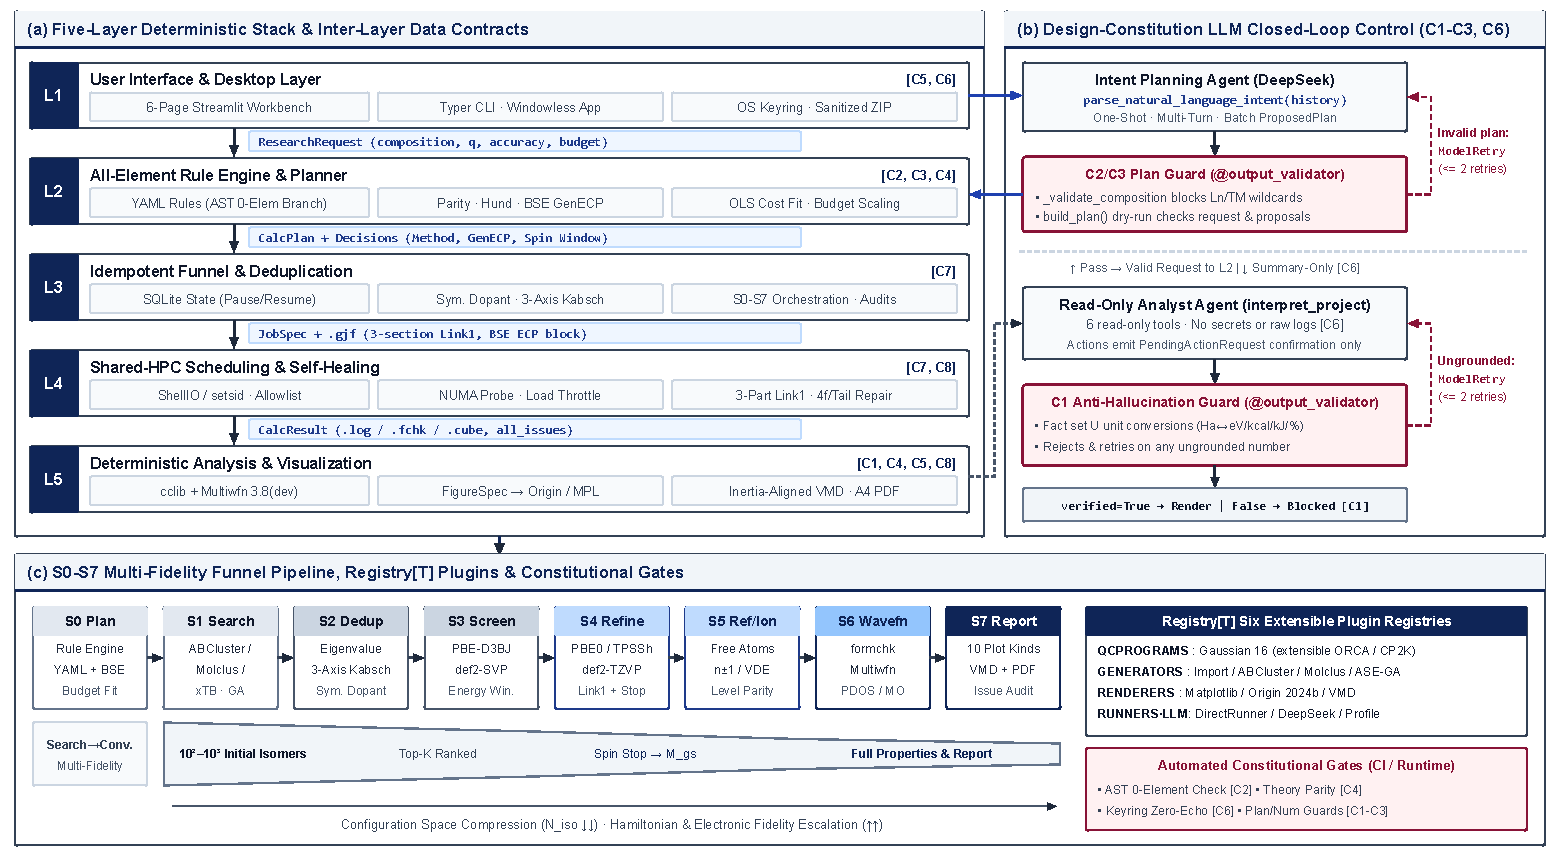
\includegraphics[width=\textwidth]{figures/fig1_architecture.pdf}
  \caption{QuantumChem AI system architecture and Design Constitution enforcement: (a) five-layer deterministic software stack and inter-layer Pydantic data contracts; (b) Design-Constitution-governed LLM closed-loop planning and read-only anti-hallucination control (C1--C3, C6); (c) S0--S7 multi-fidelity configurational funnel pipeline, \texttt{Registry[T]} plugin interfaces, and automated CI/runtime constitutional gates.}
  \label{fig:arch}
\end{figure}

Figure~\ref{fig:arch}c summarizes the idempotent S0--S7 eight-stage computational funnel managed by \texttt{PipelineWorker}:
\begin{description}
  \item[S0 (Planning \& Confirmation):] Translates \texttt{ResearchRequest} via the YAML rule engine into an auditable \texttt{CalcPlan} and Markdown proposal ready for optional parameter overrides.
  \item[S1 (Global Structural Search):] Prioritizes user-supplied coordinates, ABCluster (\texttt{isomer} + GFN2-xTB), Molclus, or an automated \texttt{ase-ga} + \texttt{tblite} GFN2-xTB fallback, combined with symmetry-unique dopant enumeration for alloy/endohedral clusters.
  \item[S2 (Geometric Deduplication \& Windowing):] Filters high-energy and spatially equivalent isomers, forwarding the top $K$ distinct representatives to DFT.
  \item[S3 (Coarse DFT Screening):] Optimizes and ranks candidate isomers and trial spin states using PBE-D3BJ/def2-SVP.\cite{perdew1996pbe,grimme2011d3bj,weigend2005def2}
  \item[S4 (High-Fidelity Refinement \& Spin Scan):] Escalates to hybrid or meta-hybrid triple-$\zeta$ DFT (PBE0-D3BJ/def2-TZVP\cite{adamo1999pbe0} or TPSSh-D3BJ/def2-TZVP\cite{staroverov2003tpssh}) under the three-section \texttt{--Link1--} protocol (\texttt{opt} $\rightarrow$ \texttt{stable=opt} $\rightarrow$ \texttt{freq}) with adaptive multiplicity pruning.
  \item[S5 (Reference \& Vertical States):] Computes level-matched isolated reference atoms, $n \pm 1$ neighbors, and ionic/vertical detachment states (VDE/ADE/VIP/VEA).\cite{jian2019pes}
  \item[S6 (Wavefunction Post-Processing):] Converts checkpoints via \texttt{formchk}, executes version-locked Multiwfn 3.8(dev)\cite{lu2012multiwfn} batch scripts for Hirshfeld/ADCH charges, atomic spin populations, projected density of states (PDOS), and frontier orbital compositions, and writes spin-density/MO \texttt{.cube} grids via \texttt{cubegen}.
  \item[S7 (Synthesis, Visualization \& Reporting):] Computes deterministic observables, generates 10 classes of 2D figures and inertia-aligned 3D renders, and compiles publication-ready A4 HTML/PDF reports.
\end{description}

\section{Core Algorithms and Implementation}

\subsection{Zero-Hardcoding Periodic Rule Engine and Adaptive Spin Scan}

The planning module (\texttt{src/qcai/planner/}) resolves arbitrary chemical compositions $\{Z_i\}$ and net charge $q$ purely through physical laws and periodic attributes:
\begin{enumerate}
  \item \textbf{Electron Parity \& Hund-Rule Atomic Multiplicities:} Given total electron count $N_e = \sum_i Z_i - q$, physically permissible spin multiplicities $M = 2S + 1$ satisfy $(N_e + M) \bmod 2 = 1$ with $M - 1 \le N_e$. Atomic reference multiplicities query ASE ground-state magnetic moments and fall back to Hund-rule \texttt{pymatgen} subshell fillings for lanthanides and heavy elements absent from default tables.
  \item \textbf{Adaptive Multiplicity Early Stopping \& Boundary Expansion:} During stage S4, initial spin windows scale by block ($d$/$f$ cap $M_{\max} \le 12$, main-group cap $\le 6$) and dynamically converge via Table~\ref{tab:alg1}: high-spin branches prune early once two consecutive states exceed the lowest converged energy by $\Delta E_{\text{stop}} = 0.50$~eV, whereas boundary minima trigger automatic expansion in steps of $\Delta M = 2$.
  \item \textbf{BSE \texttt{GenECP} Verification \& Relativistic Guards:} Prior to job emission, the Basis Set Exchange\cite{pritchard2019bse} API validates coverage across every element in the cluster. Elements lacking native built-in \texttt{def2} definitions in Gaussian 16 (such as $\mathrm{Ce\text{--}Lu}$) automatically receive explicit BSE-exported \texttt{GenECP} basis and ECP blocks, empirical dispersion keywords (\texttt{GD3}/\texttt{GD3BJ}) incompatible with superheavy actinides ($Z > 94$) are omitted cleanly, and open-shell routes apply unrestricted (\texttt{U}) prefixes with \texttt{scf=(xqc,maxcycle=500)}.
  \item \textbf{OLS Cost Calibration \& Time-Budget Contraction:} An ordinary least-squares scaling regression model updates runtime coefficients from completed runs and contracts candidate count $K$ deterministically when a wall-clock time budget is constrained.
\end{enumerate}

\begin{table}[htbp]
  \centering
  \caption{Algorithm 1: Adaptive Spin-Multiplicity Scan with Early Stopping and Boundary Expansion in Stage S4}
  \label{tab:alg1}
  \small
  \begin{tabular}{p{14.8cm}}
    \toprule
    \textbf{Input:} Pre-screened geometry $G$, electron count $N_e$, initial window $\mathcal{M}_0 = [M_{\min}, \dots, M_{\max}]$, threshold $\Delta E_{\text{stop}} = 0.50$~eV. \\
    \textbf{Output:} Converged spin-ladder results $\mathcal{R}$ and true ground-state multiplicity $M_{\text{gs}}$. \\
    \midrule
    1:\quad Initialize $\mathcal{M}$ retaining only states with $(N_e + M) \bmod 2 = 1$ and $M - 1 \le N_e$; enqueue initial batch. \\
    2:\quad \textbf{while} active jobs remain or boundary expansion is triggered \textbf{do} \\
    3:\quad \hspace{1.2em} Collect normal-termination energies $E(M)$; set $E_{\min} \leftarrow \min_M E(M)$ and $M_{\text{best}} \leftarrow \arg\min_M E(M)$. \\
    4:\quad \hspace{1.2em} \textbf{if} two consecutive states $M > M_{\text{best}}$ satisfy $E(M) - E_{\min} > \Delta E_{\text{stop}}$ \textbf{then} \\
    5:\quad \hspace{2.4em} Cancel higher-spin queued jobs (early-stop pruning) and record \texttt{Decision}. \\
    6:\quad \hspace{1.2em} \textbf{if} $M_{\text{best}} = \min(\mathcal{M})$ and $M_{\text{best}} > 2$ \textbf{then} enqueue $M_{\text{next}} = M_{\text{best}} - 2$. \\
    7:\quad \hspace{1.2em} \textbf{else if} $M_{\text{best}} = \max(\mathcal{M})$ \textbf{then} enqueue $M_{\text{next}} = M_{\text{best}} + 2$. \\
    8:\quad \textbf{return} $M_{\text{gs}} = \arg\min_M E(M)$ and complete ladder $\mathcal{R}$. \\
    \bottomrule
  \end{tabular}
\end{table}

\subsection{Symmetry Dopant Enumeration and Three-Stage Geometric Deduplication}

For doped and bimetallic clusters (\texttt{src/qcai/structure/dopant\_sites.py}), \texttt{PointGroupAnalyzer}\cite{ong2013pymatgen} partitions host atomic positions into symmetry-equivalent orbits, emitting exactly one representative per orbit for single substitution (e.g., 1 trial configuration for $O_h$ or $I_h$ hosts) and symmetry-canonicalized combinations for multi-site doping, plus centroid cavity estimation for endohedral placement.

Standard single-axis alignment in \texttt{pymatgen.HungarianOrderMatcher} yields spurious $1.7\text{--}1.9$~\AA\ RMSDs for rotated cluster isomers sharing nearly isotropic moments of inertia. The deduplication module (\texttt{src/qcai/structure/dedup.py}) resolves this via a three-stage invariant pipeline:
\begin{enumerate}
  \item \textbf{Distance-Matrix Eigenvalue Fingerprinting:} Within each energy window, $\mathcal{O}(N^3)$ sorted eigenspectra of pairwise interatomic distance matrices provide exact rotation-, translation-, and permutation-invariant pre-screening.
  \item \textbf{Tri-Axial Principal-Inertia Alignment + Hungarian/Kabsch Matching:} Candidates are transformed to mass-weighted principal-inertia frames across all four proper right-handed sign flips; optimal per-element atom assignment via the Hungarian algorithm\cite{kuhn1955hungarian} (\texttt{scipy.optimize.linear\_sum\_assignment}) followed by optimal Kabsch rotation\cite{kabsch1976} minimizes the exact RMSD.
  \item \textbf{Degenerate-Axis Fallback:} Near-spherical polyhedra whose borderline RMSDs remain close to the equivalence cutoff invoke \texttt{GeneticOrderMatcher} or \texttt{BruteForceOrderMatcher}. Across 6--38 atom benchmarks, identical rotated/translated/permuted clusters deduplicate to $10^{-15}$~\AA\ RMSD in $< 8$~ms per comparison.
\end{enumerate}

\subsection{Resilient Shared-HPC Scheduling and Server-Side \texttt{custodian} Self-Healing}

The remote execution layer (\texttt{src/qcai/remote/} and \texttt{src/qcai\_remote/}) enforces strict path confinement within \texttt{work\_root} and command allowlisting over Fabric SSH:
\begin{itemize}
  \item \textbf{NUMA Topology Probing, Load Courtesy, and Elastic Core Scaling:} \texttt{qcai\_remote/probe.py} fuses \texttt{psutil}, \texttt{lscpu -J}, and \texttt{ps -eo user,pcpu,comm} to determine NUMA socket core counts, free RAM, and competing user CPU load. \texttt{ResourceManager} pins jobs within a single NUMA node, halts new submissions (\texttt{allowed\_new\_jobs = 0}) when shared nodes are busy, and enables elastic NUMA core scaling so queued S4 jobs dynamically expand from 4 to 10--16 cores (with scaled \texttt{\%mem}) as earlier jobs drain.
  \item \textbf{Reconnect Resilience \& Anti-Race Polling:} The SSH transport maintains 30~s keepalive heartbeats and automatically reconnects dropped channels during multi-day runs. Remote background launches isolate subshell standard input to prevent hanging file descriptors, \texttt{DirectRunner} excludes stale checkpoint artifacts prior to resubmission, and completion polling re-reads \texttt{status.json} immediately upon process exit to eliminate check-vs-exit race conditions while surfacing unresolved failures to the dashboard.
  \item \textbf{Three-Section \texttt{--Link1--} \& Lossless 4f/Tail Repair:} Because Gaussian 16 rejects co-located \texttt{opt} and \texttt{stable=opt} keywords (\texttt{Illegal IType}), the writer splits refinement jobs into three sequential \texttt{--Link1--} sections (\texttt{opt} $\rightarrow$ \texttt{stable=opt geom=allcheck guess=read} $\rightarrow$ \texttt{freq geom=allcheck guess=read}). On the compute server, a hardened \texttt{custodian} error handler guards against truncated frequency and bare-route parsing crashes, monotonic SCF escalation steps open-shell $4f$ convergence protocols without repeating exhausted settings (\texttt{xqc+vshift=500+\allowbreak{}fermi+novaracc} $\rightarrow$ \texttt{xqc+vshift=800+\allowbreak{}fermi+novaracc+ndamp=30} $\rightarrow$ \texttt{vshift=1000+\allowbreak{}fermi+novaracc+ndamp=40}), lossless tail restoration preserves trailing \texttt{GenECP} and \texttt{--Link1--} blocks across automated rewrites, and \texttt{ImaginaryFreqHandler} (\texttt{step\_scale=0.25}) and \texttt{InstabilityHandler} drive saddle points and unstable wavefunctions to verified local minima.
\end{itemize}

\subsection{Deterministic Energetics and Version-Locked Multiwfn Parsing}

Under Articles C1 and C4, \texttt{src/qcai/analysis/} evaluates all cluster energetic, electronic, and magnetic descriptors via unit-tested equations:
\begin{align}
  E_b &= \frac{\sum_k n_k E(\text{atom}_k) - E(\text{cluster})}{N} \label{eq:eb} \\
  \Delta_2 E(n) &= E(n+1) + E(n-1) - 2E(n) \label{eq:d2e} \\
  E_f &= E(A) + E(B) - E(AB) \label{eq:ef} \\
  E_{\text{emb}} &= E(\text{Host}) + E(\text{Dopant}) - E(\text{Host+Dopant}) \label{eq:eemb} \\
  E_{\text{sub}} &= E(\text{Host}_{n-1}D) + E(\text{Host}_{\text{atom}}) - E(\text{Host}_n) - E(D) \label{eq:esub} \\
  \Delta(A_m B_n) &= E(A_m B_n) - \frac{m}{m+n}E(A_{m+n}) - \frac{n}{m+n}E(B_{m+n}) \label{eq:mix} \\
  \text{VDE} &= E_{\text{neu}}(\mathbf{R}_{\text{an}}) - E_{\text{an}}(\mathbf{R}_{\text{an}}), \qquad
  \text{ADE} = E_{\text{neu}}(\mathbf{R}_{\text{neu}}) - E_{\text{an}}(\mathbf{R}_{\text{an}}) \label{eq:pes} \\
  f_D &= \frac{\sum_{i \in D}|s_i|}{\sum_{\text{all } j}|s_j|} \label{eq:fd}
\end{align}
Jellium valence-electron counts automatically flag closed-shell superatom magic numbers ($2, 8, 18, 20, 34, 40, 58, 92$), while significant spin contamination triggers an explicit warning whenever $|\langle S^2 \rangle - S(S+1)| / S(S+1) > 10\%$ (and $|\Delta \langle S^2 \rangle| > 0.1$).

Because Multiwfn interactive menus evolve across builds, \texttt{src/qcai/programs/multiwfn/} enforces a strict version lock verifying the output banner against tested \texttt{Version 3.8(dev) (2025-Mar-10)}, raising \texttt{MultiwfnVersionError} on mismatch. Fixed-width Fortran negative-sign concatenations in \texttt{DOS\_curve.txt} are cleanly separated via regex preprocessing (\texttt{(?<=\textbackslash d)-}), enabling automated extraction of Hirshfeld/ADCH charges (menu \texttt{7->1/11}), atomic spin populations (\texttt{15->-1->3->1->5}), element- and angular-momentum-resolved PDOS (\texttt{10}), and frontier orbital shares (\texttt{8->1}).

\subsection{Dual-Engine Visualization and Anti-Hallucination LLM Layer}

\texttt{FigureSpec} cleanly feeds ten standard plot schemas (\texttt{levels}, \texttt{levels\_compare}, \texttt{spin}, \texttt{dos}, \texttt{orb\_comp}, \texttt{spin\_ladder}, \texttt{isomer\_ranking}, \texttt{size\_evolution}, \texttt{vde\_ade}, and \texttt{s2}) to both Matplotlib and a serialized Windows Origin 2024b subprocess outputting PNG, SVG, and editable \texttt{.opju} workbooks (using custom \texttt{.otpu} templates and built-in \texttt{PAN4} four-panel grids for size evolution). Simultaneously, \texttt{align\_cluster\_principal\_axes} locks both interactive web \texttt{py3Dmol} views and headless VMD (\texttt{Orthographic} + \texttt{TachyonInternal}) ray-traced scenes onto identical inertia-aligned viewpoints prior to Playwright A4 PDF report compilation.

Within \texttt{src/qcai/ai/}, two separated \texttt{pydantic-ai} agents collaborate under constitutional guardrails:
\begin{enumerate}
  \item \textbf{Intent-to-Plan Agent with Dry-Run Validator:} Input composition validation rejects generic group wildcards (\texttt{Ln}, \texttt{TM}, \texttt{M}) prior to planning. The intent-parser output validator executes \texttt{build\_plan()} as a deterministic dry run on both the direct request and every proposed candidate plan, issuing automatic schema-repair retries when constraints fail. Explicit requests advance directly to plan review, follow-up turns merge prior conversation context consistently, and family-level queries generate selectable or batch-submittable (up to 10) executable proposals.
  \item \textbf{Read-Only Analyst with Unit-Conversion Grounding Guard:} The analytical interpreter exposes only six read-only query tools plus one non-mutating confirmation-request tool. Its output validator gathers observed fact values, expands valid equivalence sets across Hartree $\leftrightarrow$ eV ($27.211386$~eV/Ha), kcal/mol ($627.509474$), kJ/mol ($2625.49964$), and percentages, triggers up to two schema-repair retries on ungrounded figures, and flags unverified responses to block display in the interface.
\end{enumerate}

\section{Validation and Production Case Studies}

\subsection{Ten Reference Gaussian 16 Benchmarks}

Ten reference Gaussian 16 calculations spanning $s$-block, $p$-block superatoms, $3d$ high-spin, $5d$ endohedral \texttt{GenECP}, bimetallic alloys, doped open-shell clusters, two-section \texttt{Link1} stability checks, and four intentional fault-injection scenarios were executed on remote Linux compute nodes via \texttt{DirectRunner} and archived in \texttt{tests/data/golden/}. Table~\ref{tab:golden} summarizes parsed observables and server-side \texttt{custodian} outcomes; Figure~\ref{fig:vmd} shows VMD ray-traced 3D structures for the six converged chemical clusters, and Figure~\ref{fig:gaps} compares their HOMO--LUMO gaps.

\begin{table}[htbp]
  \centering
  \caption{Parsed Observables and Server-Side \texttt{custodian} Recovery Outcomes for Ten Reference Gaussian 16 Benchmarks}
  \label{tab:golden}
  \scriptsize
  \setlength{\tabcolsep}{3.2pt}
  \resizebox{\textwidth}{!}{%
  \begin{tabular}{@{}llccrrccc@{}}
    \toprule
    ID & System ($N$) & $q/M$ & Status & $E_{\text{SCF}}$ (Ha) & $E_{\mathrm{g}}$ (eV) & $\langle S^2 \rangle$ (Ideal) & $n_{\text{imag}}$ / Stable & Server-Side Recovery Outcome \\
    \midrule
    \texttt{na6} & $\mathrm{Na_6}$ (6) & 0 / 1 & \texttt{done} & $-972.741909$ & 1.090 & --- & 0 / --- & $s$-block closed-shell convergence \\
    \texttt{al13\_anion} & $\mathrm{Al_{13}^-}$ (13) & $-1$ / 1 & \texttt{done} & $-3149.265871$ & 1.952 & --- & 0 / --- & 40$\mathrm{e}^-$ closed-shell superatom \\
    \texttt{fe4} & $\mathrm{Fe_4}$ (4) & 0 / 13 & \texttt{done} & $-5053.212837$ & 0.259 & 42.0214 (42.00) & 0 / --- & $3d$ high-spin; low spin contamination \\
    \texttt{w\_au12} & $\mathrm{W@Au_{12}}$ (13) & 0 / 1 & \texttt{done} & $-1696.516466$ & 3.337 & --- & 0 / --- & BSE \texttt{GenECP} 18$\mathrm{e}^-$ icosahedral shell \\
    \texttt{cu3ag3} & $\mathrm{Cu_3Ag_3}$ (6) & 0 / 1 & \texttt{done} & $-5361.213378$ & 1.908 & --- & 0 / --- & Bimetallic mixed basis/ECP convergence \\
    \texttt{al12cu} & $\mathrm{Al_{12}Cu}$ (13) & 0 / 2 & \texttt{done} & $-4546.981501$ & 0.277 & 0.8047 (0.75) & 0 / --- & \texttt{ImaginaryFreqHandler} resolved Jahn--Teller \\
    \texttt{fault\_imag\_freq} & $\mathrm{Au_4}$ saddle (4) & 0 / 1 & \texttt{done} & $-543.167628$ & 0.990 & --- & 0 / --- & Displaced along normal mode (\texttt{scale=0.25}) \\
    \texttt{fault\_opt\_maxsteps} & L9999 test (3) & 0 / 2 & \texttt{done} & $-3427.042431$ & 0.257 & 0.7500 (0.75) & 0 / --- & Step-limit handler resumed \& converged \\
    \texttt{fault\_scf\_noconv} & L502 test (4) & 0 / 5 & \texttt{failed} & $-5052.846030$ & --- & 8.4967 (6.00) & 0 / --- & Escalated \texttt{maxcycle=100}/\texttt{xqc}; flagged \texttt{needs\_human} \\
    \texttt{link1\_stable\_opt} & Link1 test (2) & 0 / 3 & \texttt{done} & $-3015.648103$ & 2.287 & 2.0013 (2.00) & 0 / \texttt{True} & 2-section Link1 parsed; \texttt{stable=True} \\
    \bottomrule
  \end{tabular}%
  }
\end{table}

\begin{figure}[htbp]
  \centering
  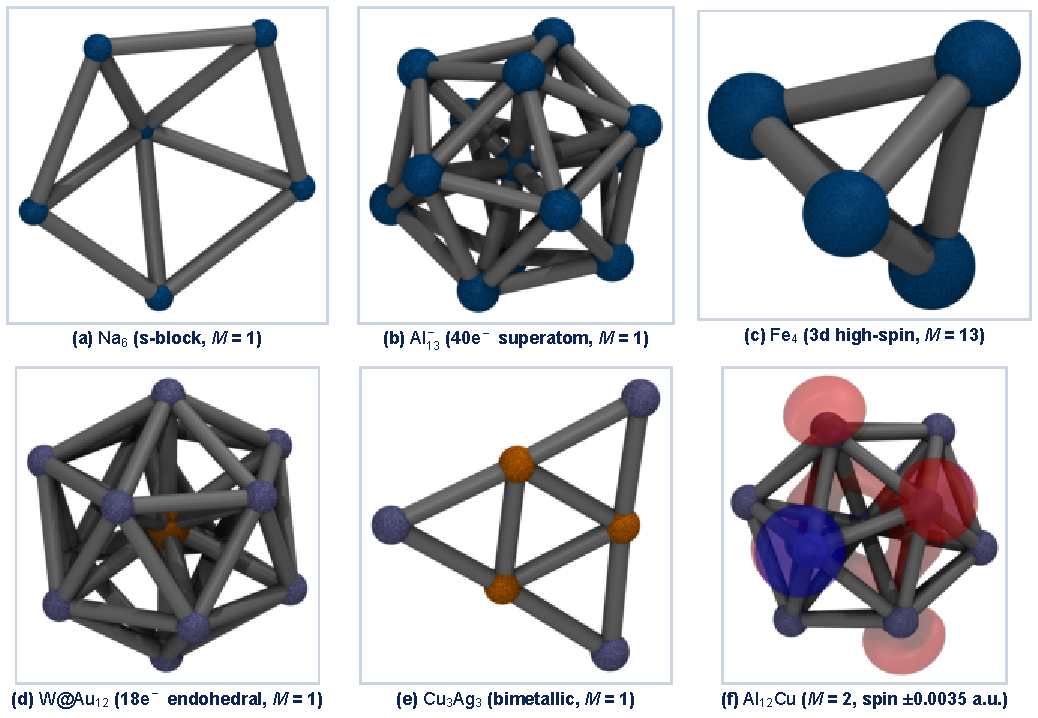
\includegraphics[width=0.92\textwidth]{figures/fig2_golden_3d_vmd.pdf}
  \caption{Principal-inertia-aligned 3D cluster geometries rendered via VMD (\texttt{TachyonInternal}) across six converged reference benchmarks: (a) $\mathrm{Na_6}$, (b) $\mathrm{Al_{13}^-}$, (c) $\mathrm{Fe_4}$, (d) $\mathrm{W@Au_{12}}$, (e) $\mathrm{Cu_3Ag_3}$, and (f) $\mathrm{Al_{12}Cu}$ overlaid with Multiwfn real-space spin density isosurfaces at $\pm 0.0035$~a.u. (red: $+\alpha$; blue: $-\beta$ polarization).}
  \label{fig:vmd}
\end{figure}

\begin{figure}[htbp]
  \centering
  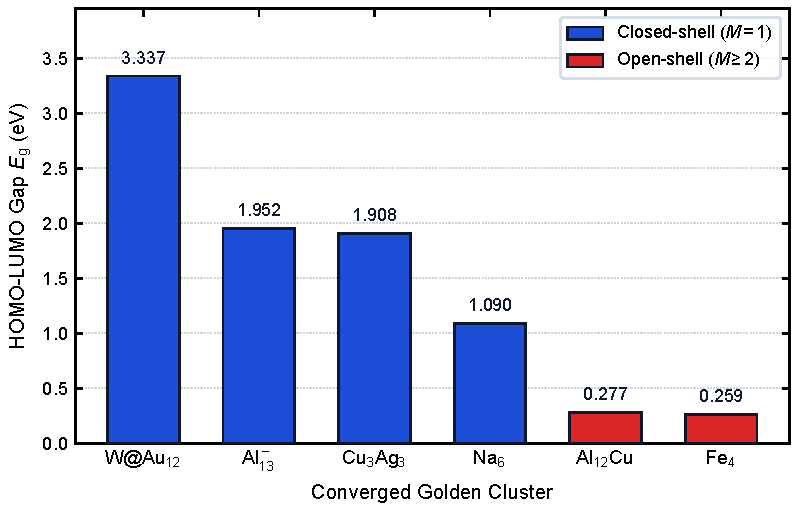
\includegraphics[width=0.72\textwidth]{figures/fig3_golden_gaps.pdf}
  \caption{HOMO--LUMO gaps ($E_{\mathrm{g}}$, eV) across six converged reference benchmarks spanning $s$-, $p$-, $3d$-, and $5d$-block clusters (blue: closed-shell singlets $M=1$; red: open-shell magnetic/doped systems $M \ge 2$).}
  \label{fig:gaps}
\end{figure}

Across the converged systems, magic-number closed-shell $\mathrm{W@Au_{12}}$ ($18\mathrm{e}^-$, $I_h$ cage, $E_{\mathrm{g}} = 3.337$~eV), $\mathrm{Al_{13}^-}$ ($40\mathrm{e}^-$, 1.952~eV), and planar triangular $\mathrm{Cu_3Ag_3}$ (1.908~eV) exhibit wide frontier gaps, whereas high-spin $\mathrm{Fe_4}$ ($M=13$, $\langle S^2 \rangle = 42.0214$, 0.259~eV) and doublet $\mathrm{Al_{12}Cu}$ ($M=2$, 0.277~eV) show narrower HOMO--LUMO gaps driven by open-shell valence states. Every recoverable fault scenario converged autonomously without human intervention, while the non-convergent SCF stress test (\texttt{fault\_scf\_noconv}) exhausted escalation safely, set \texttt{needs\_human=True}, and exposed its spin contamination ($\langle S^2 \rangle = 8.4967$ vs ideal 6.00).

\subsection{$\mathrm{Al_{12}Cu}$ Multiwfn Wavefunction Analysis}

Stage S6--S7 post-processing on $\mathrm{Al_{12}Cu}$ ($q=0, M=2$, 37 valence electrons) extracted Hirshfeld/ADCH charges, Hirshfeld atomic spin populations, a 3,000-point PDOS spectrum ($-21.77$ to $+5.44$~eV), and frontier orbital angular-momentum decompositions (Table~\ref{tab:al12cu}, Figures~\ref{fig:al12cu_elec} and~\ref{fig:al12cu_spin}).

\begin{table}[htbp]
  \centering
  \caption{Quantitative Electronic and Spin Observables of $\mathrm{Al_{12}Cu}$ Extracted via Version-Locked Multiwfn 3.8(dev)}
  \label{tab:al12cu}
  \footnotesize
  \resizebox{\textwidth}{!}{%
  \begin{tabular}{@{}llll@{}}
    \toprule
    Analysis Item & Observable & Measured Value & Physical Interpretation \\
    \midrule
    Cu Charge Population & Hirshfeld / ADCH & $+0.1597\,e$ / $-0.0086\,e$ & Mild covalent hybridization between Cu and $\mathrm{Al_{12}}$ cage \\
    Hirshfeld Spin Density & $\mathrm{spin(Cu)}$ / $\sum s_i$ / $\sum |s_i|$ & $+0.0809\,e$ / $+1.0000\,e$ / $2.0694\,e$ & Net spin conserved; $f_D(\mathrm{Cu}) = 3.91\%$ (cage-delocalized) \\
    MO 93 (HOMO-$\alpha$) & Energy / $s$-$p$-$d$ (\%) / Cu (\%) & $-5.046$~eV / 18.09, 78.53, 3.37 / 17.41 & Dominated by Al $3p$ hybridized with Cu valence states \\
    MO 339 (HOMO-$\beta$) & Energy / $s$-$p$-$d$ (\%) / Cu (\%) & $-4.987$~eV / 19.45, 77.21, 3.35 / 17.68 & Symmetrical frontier character across $\alpha$/$\beta$ channels \\
    MO 94 (LUMO-$\alpha$) & Energy / $s$-$p$-$d$ (\%) / Cu (\%) & $-4.655$~eV / 24.89, 71.47, 3.65 / 15.75 & Narrow-gap open-shell acceptor (overall $E_{\mathrm{g}} = 0.277$~eV) \\
    MO 340 (LUMO-$\beta$) & Energy / $s$-$p$-$d$ (\%) / Cu (\%) & $-4.710$~eV / 20.58, 75.62, 3.80 / 16.70 & Confirms Al $3s/3p$ conduction-edge dominance \\
    \bottomrule
  \end{tabular}%
  }
\end{table}

\begin{figure}[htbp]
  \centering
  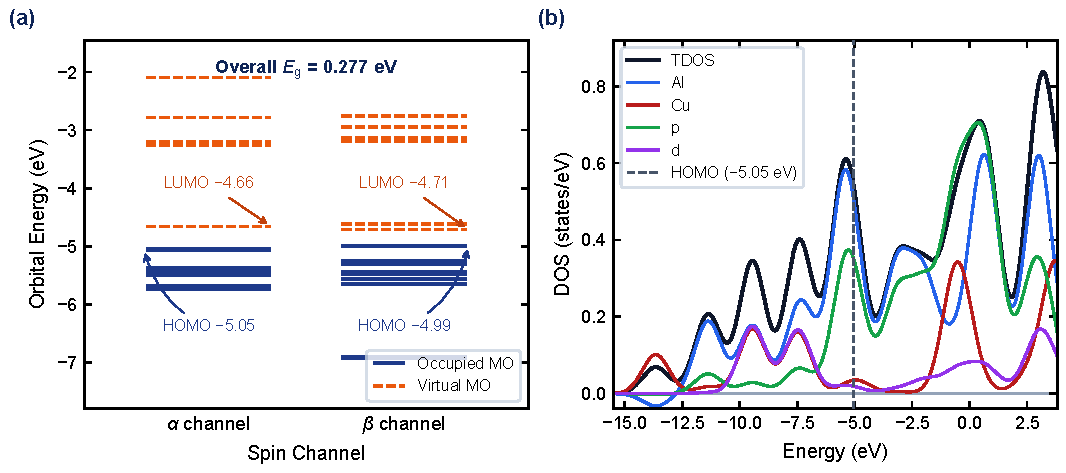
\includegraphics[width=\textwidth]{figures/fig4_al12cu_electronic.pdf}
  \caption{Electronic structure of $\mathrm{Al_{12}Cu}$ ($M=2$) parsed from Gaussian 16 and Multiwfn 3.8(dev): (a) spin-polarized $\alpha$ and $\beta$ frontier molecular orbital levels (solid blue: occupied; dashed orange: virtual); (b) TDOS and Al, Cu, $p$, and $d$ projected density of states curves with vertical dashed line marking $\alpha$-HOMO ($-5.05$~eV).}
  \label{fig:al12cu_elec}
\end{figure}

\begin{figure}[htbp]
  \centering
  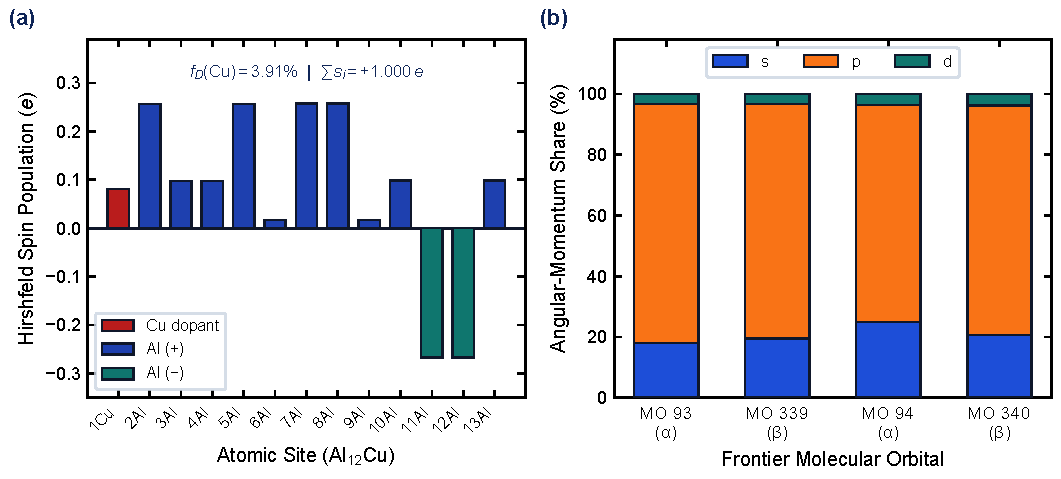
\includegraphics[width=\textwidth]{figures/fig5_al12cu_spin_orb.pdf}
  \caption{Spin polarization and orbital bonding distribution in $\mathrm{Al_{12}Cu}$: (a) atomic Hirshfeld spin populations across all 13 sites demonstrating $f_D(\mathrm{Cu}) = 3.91\%$ and antiparallel $-0.267\,e$ polarization on \texttt{11Al}/\texttt{12Al} matching the blue isosurface lobe in Figure~\ref{fig:vmd}f; (b) $s$/$p$/$d$ angular-momentum decomposition across frontier $\alpha$/$\beta$ orbitals.}
  \label{fig:al12cu_spin}
\end{figure}

The unpaired electron delocalizes extensively across the $\mathrm{Al_{12}}$ host ($f_D(\mathrm{Cu}) = 3.91\%$), inducing symmetric antiparallel spin polarization ($-0.2673\,e$ and $-0.2674\,e$) on two opposite aluminum vertices (\texttt{11Al}, \texttt{12Al}) that matches the negative $\beta$-spin lobe rendered by VMD in Figure~\ref{fig:vmd}f.

\subsection{Bilingual 50+50 Scientific Instruction Evaluation and Anti-Hallucination Verification}

To evaluate natural-language automation rigorously without linguistic bias, the \texttt{pydantic-ai} intent planner was evaluated against two paired 50-instruction suites spanning every periodic-table block, bimetallic and endohedral doping, size-evolution ranges, charged ions, all six recipes, three accuracy tiers, explicit time budgets, and 8 deliberately underspecified clarification prompts: the original Chinese suite (\texttt{tests/llm\_eval/instructions.yaml}) and a matched English suite (\texttt{tests/llm\_eval/instructions\_en.yaml}). Executed live via \texttt{eval\_runner.py} against an OpenAI-compatible DeepSeek endpoint (\texttt{deepseek-v4.1-flash}), both benchmarks achieved 50/50 (100.0\%) accuracy (Table~\ref{tab:bilingual}), passing the $\ge 90\%$ \texttt{pytest -m llm} acceptance threshold.

\begin{table}[htbp]
  \centering
  \caption{Category-Level Bilingual Natural-Language-to-Plan Evaluation on \texttt{deepseek-v4.1-flash} (50 Chinese + 50 Matched English Scientific Instructions)}
  \label{tab:bilingual}
  \footnotesize
  \setlength{\tabcolsep}{4pt}
  \resizebox{\textwidth}{!}{%
  \begin{tabular}{@{}lccccc@{}}
    \toprule
    Benchmark Category & Case Count & Chinese Pass & Chinese Accuracy & English Pass & English Accuracy \\
    \midrule
    $s$-block clusters & 6 & 6/6 & 100.0\% & 6/6 & 100.0\% \\
    $p$-block clusters (incl.\ anions) & 8 & 8/8 & 100.0\% & 8/8 & 100.0\% \\
    $3d$ transition-metal \& doped & 12 & 12/12 & 100.0\% & 12/12 & 100.0\% \\
    $4d$/$5d$ \& bimetallic / endohedral & 13 & 13/13 & 100.0\% & 13/13 & 100.0\% \\
    Lanthanide ($4f$) doped & 3 & 3/3 & 100.0\% & 3/3 & 100.0\% \\
    Ambiguous (clarification required) & 8 & 8/8 & 100.0\% & 8/8 & 100.0\% \\
    \midrule
    \textbf{Total} & \textbf{50} & \textbf{50/50} & \textbf{100.0\%} & \textbf{50/50} & \textbf{100.0\%} \\
    \bottomrule
  \end{tabular}%
  }
\end{table}

On exploratory family-level queries (such as ``electronic structural rigidity in heavy lanthanide endohedral gold pentamer superatoms''), the planner triggers \texttt{ProposedPlan} generation across representative concrete compositions (\texttt{Lu@Au5}, \texttt{Gd@Au5}, \texttt{Yb@Au5}) or expands the full 8-element series into independent executable projects with zero element-placeholder leakage. Offline adversarial tests in \texttt{tests/unit/test\_ai\_layer.py} further verify unit-conversion equivalence pass-through, \texttt{ModelRetry} rejection of fabricated numbers, and UI blocking when retries exhaust.

\subsection{Autonomous Heavy Lanthanide $\mathrm{Ln@Au_5}$ Production Study}

To evaluate unattended multi-day scientific throughput on a shared Linux cluster, an exploratory natural-language prompt initiated batch submission of all eight heavy lanthanide systems ($\mathrm{Ln@Au_5}$, $\mathrm{Ln} = \mathrm{Gd\text{--}Lu}$) alongside an independent standalone $\mathrm{Tm@Au_5}$ reproduction (\texttt{proj\_a9065c59}). Across 9 projects and 230 pipeline jobs comprising 221 real Gaussian 16 runs (18 \texttt{S0} \texttt{PBE0-D3BJ/def2-TZVP} free atoms, 184 \texttt{S3} \texttt{PBE-D3BJ/def2-SVP} isomer/multiplicity screens, and 19 \texttt{S4} three-section \texttt{--Link1--} \texttt{PBE0-D3BJ/def2-TZVP} refinements using BSE \texttt{GenECP}), the platform logged 442.76 wall-clock hours (1,399.78 CPU core-hours) and achieved 100\% convergence (230/230 jobs, 0 failures). During tail execution, elastic NUMA scaling dynamically upgraded \texttt{S4} jobs from 4 cores to 10 cores (1 job) and 16 cores (2 jobs), while server-side \texttt{custodian} resolved 7 open-shell $4f$ faults autonomously (5 lossless SCF escalations across \texttt{Tb}/\texttt{Dy}/\texttt{Er}, 1 imaginary-mode perturbation on \texttt{Tb S4 ($M=9$)}, and 1 step-limit continuation on \texttt{Dy S4 ($M=6$)}). All 19 \texttt{S4} isomers passed \texttt{n\_imag = 0} and \texttt{stable = True}.

\begin{table}[htbp]
  \centering
  \caption{Ground-State Properties (\texttt{PBE0-D3BJ/def2-TZVP}, BSE \texttt{GenECP}) and Compute Statistics Across Heavy Lanthanide $\mathrm{Ln@Au_5}$ ($\mathrm{Ln} = \mathrm{Gd\text{--}Lu}$)}
  \label{tab:lnau5}
  \scriptsize
  \setlength{\tabcolsep}{3.0pt}
  \resizebox{\textwidth}{!}{%
  \begin{tabular}{@{}llcrrcrcccc@{}}
    \toprule
    System ($Z$) & Project ID & $M_{\text{gs}}$ ($\mu_{\mathrm{B}}$) & $E_{\text{SCF}}$ (Ha) & $E_b$ (eV/at.) & $E_{\mathrm{g}}$ (eV) & $\langle S^2 \rangle$ (Ideal) & PG & $d_{\text{avg}}$(Ln--Au) (\AA) & $q_{\text{APT}}$ / spin(Ln) & Core$\cdot$h / Fixes \\
    \midrule
    $\mathrm{Gd@Au_5}$ (64) & \texttt{proj\_2c89192f} & 8 (7) & $-1444.567777$ & 1.992 & 1.679 & 15.7687 (15.75) & $C_s$ & $2.934\pm 0.107$ & $+0.44$ / $+7.74$ & 90.44 / 0 \\
    $\mathrm{Tb@Au_5}$ (65) & \texttt{proj\_19154707} & 7 (6) & $-1503.335694$ & 2.408 & 2.665 & 12.0105 (12.00) & $C_s$ & $2.827\pm 0.089$ & $+0.97$ / $+6.16$ & 109.88 / 2 \\
    $\mathrm{Dy@Au_5}$ (66) & \texttt{proj\_7a0ee451} & 6 (5) & $-1563.991806$ & 2.291 & 2.702 & 8.7572 (8.75) & $C_s$ & $2.815\pm 0.089$ & $+0.94$ / $+5.05$ & 595.42 / 3 \\
    $\mathrm{Ho@Au_5}$ (67) & \texttt{proj\_fc156187} & 5 (4) & $-1627.180455$ & 1.969 & 2.754 & 6.0000 (6.00) & $C_{2v}$ & $2.827\pm 0.160$ & $+1.15$ / $+4.10$ & 24.69 / 0 \\
    $\mathrm{Er@Au_5}$ (68) & \texttt{proj\_fa892f93} & 4 (3) & $-1694.269982$ & 2.025 & 2.709 & 3.7500 (3.75) & $C_s$ & $2.791\pm 0.080$ & $+0.92$ / $+3.06$ & 490.10 / 2 \\
    $\mathrm{Tm@Au_5}$ (69) & \texttt{proj\_735cfc68} & 3 (2) & $-1764.511111$ & 1.800 & 2.524 & 2.0000 (2.00) & $C_{2v}$ & $2.805\pm 0.150$ & $+1.11$ / $+2.04$ & 19.21 / 0 \\
    $\mathrm{Yb@Au_5}$ (70) & \texttt{proj\_51ac0f99} & 2 (1) & $-1838.137089$ & 1.802 & 1.499 & 0.7501 (0.75) & $C_s$ & $2.928\pm 0.016$ & $+0.57$ / $+0.18$ & 46.92 / 0 \\
    $\mathrm{Lu@Au_5}$ (71) & \texttt{proj\_9f91b2dc} & 1 (0) & $-1915.063709$ & 2.248 & 2.812 & --- & $C_{2v}$ & $2.782\pm 0.143$ & $+1.06$ / $0.00$ & 4.22 / 0 \\
    \bottomrule
  \end{tabular}%
  }
\end{table}

\begin{figure}[htbp]
  \centering
  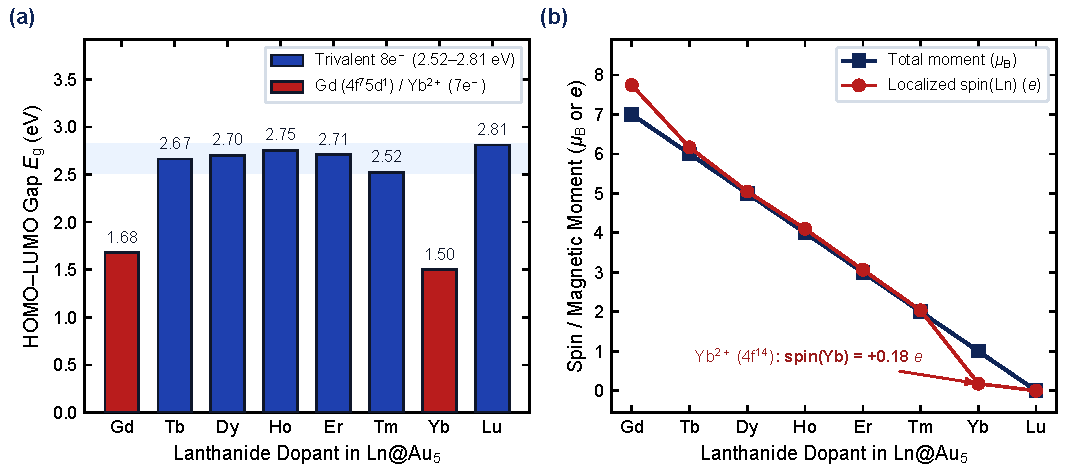
\includegraphics[width=\textwidth]{figures/fig6_ln_au5_rigidity.pdf}
  \caption{Electronic rigidity and $4f$ spin decoupling across $\mathrm{Ln@Au_5}$ ($\mathrm{Ln} = \mathrm{Gd\text{--}Lu}$) at \texttt{PBE0-D3BJ/def2-TZVP (GenECP)}: (a) trivalent $8\mathrm{e}^-$ superatom HOMO--LUMO gap rigidity plateau ($2.524\text{--}2.812$~eV for Tb--Tm, Lu) contrasted against $\mathrm{Gd}$ ($4f^7 5d^1$) and divalent $\mathrm{Yb^{2+}}$ ($4f^{14}$, $7\mathrm{e}^-$) drops; (b) total spin magnetic moment $\mu$ ($\mu_{\mathrm{B}}$) versus localized lanthanide Mulliken spin $\mathrm{spin(Ln)}$ ($e$), confirming localized $4f$ spin behavior for Tb--Tm and abrupt spin delocalization onto the $\mathrm{Au_5}$ host in $\mathrm{Yb@Au_5}$.}
  \label{fig:lnau5}
\end{figure}

Table~\ref{tab:lnau5} and Figure~\ref{fig:lnau5} reveal three clear physical regimes:
\begin{enumerate}
  \item \textbf{Trivalent $8\mathrm{e}^-$ Superatom Rigidity Plateau:} Across Tb, Dy, Ho, Er, Tm, and Lu, trivalent $\mathrm{Ln^{3+}}$ donates three valence electrons to the $\mathrm{Au_5}$ framework ($5\times 1 + 3 = 8\mathrm{e}^-$ closed superatom shell), locking $E_{\mathrm{g}}$ within a rigid $2.524\text{--}2.812$~eV plateau alongside monotonic lanthanide contraction ($d_{\text{avg}}(\text{Ln--Au})$: $2.827 \rightarrow 2.782$~\AA) and high positive charge transfer ($q_{\text{APT}} = +0.92$ to $+1.15$).
  \item \textbf{Localized $4f$ Spin Decoupling:} From Tb to Tm, total magnetic moment decreases monotonically ($6 \rightarrow 2\,\mu_{\mathrm{B}}$) while remaining strictly localized on the lanthanide core ($\mathrm{spin(Ln)} = +6.16 \rightarrow +2.04\,e$) with minimal spin contamination ($|\langle S^2 \rangle - S(S+1)| \le 0.011$), demonstrating electronic decoupling between core $4f^n$ spins and the $8\mathrm{e}^-$ superatom valence shell.
  \item \textbf{Divalent $\mathrm{Yb^{2+}}$ Transition \& Inter-Run Reproducibility:} Driven by stability of the filled $4f^{14}$ subshell, $\mathrm{Yb@Au_5}$ adopts a divalent $\mathrm{Yb^{2+}}$ ($7\mathrm{e}^-$ open-shell) configuration, expanding $d_{\text{avg}}(\text{Yb--Au})$ to $2.928$~\AA, reducing $q_{\text{APT}}$ to $+0.57$, collapsing $E_{\mathrm{g}}$ to $1.499$~eV, and shifting the unpaired spin onto the $\mathrm{Au_5}$ host (only $+0.18\,e$ remaining on Yb). Furthermore, independent reproduction \texttt{proj\_a9065c59} ($\mathrm{Tm@Au_5}$, $E_{\text{SCF}} = -1764.510373$~Ha, $E_{\mathrm{g}} = 2.521$~eV) matches batch project \texttt{proj\_735cfc68} within $0.0007$~Ha and $0.003$~eV.
\end{enumerate}

\subsection{Software Engineering, Five-Tier Verification, and Desktop Workbench Delivery}

QuantumChem AI comprises 75 Python modules under \texttt{src/}, 11 Streamlit UI modules under \texttt{web/}, and a five-tier verification pyramid (Table~\ref{tab:tests}). All source files pass \texttt{ruff} formatting/linting, strict \texttt{mypy src} type checking, AST zero-element-branch scanning, and 115 automated offline unit and headless Playwright E2E browser tests.

\begin{table}[htbp]
  \centering
  \caption{Five-Tier Automated Verification Pyramid of QuantumChem AI}
  \label{tab:tests}
  \footnotesize
  \resizebox{\textwidth}{!}{%
  \begin{tabular}{@{} >{\raggedright\arraybackslash}p{2.3cm} >{\raggedright\arraybackslash}p{4.7cm} >{\raggedright\arraybackslash}p{3.3cm} >{\raggedright\arraybackslash}p{3.9cm} @{}}
    \toprule
    Tier & Verification Scope & Observed Status & Representative Modules / Gates \\
    \midrule
    L1: Static \& Constitution & \texttt{ruff}, \texttt{mypy src}, AST 0-element check, \texttt{Hypothesis} tests & 75 files typed; 0 AST violations & \texttt{test\_axiom\_no\_\allowbreak{}element\_\allowbreak{}branches.py} \\
    L2: Offline Unit & Energetics, SCF/tail repair, BSE \texttt{GenECP}, 3-axis dedup, guards & 113 unit tests passed (115 total offline) & \texttt{tests/unit/*.py} \\
    L3: Local Renderers & Origin 2024b (incl.\ \texttt{PAN4}, $\mathrm{Ln@Au_5}$) \& VMD ray tracing & 6 Origin tests + VMD render passed & \texttt{test\_origin\_\allowbreak{}renderer.py} \\
    L4: HPC \& Live AI & Linux SSH probe, 10 reference runs, 230-job $\mathrm{Ln@Au_5}$, 50+50 eval & 100\% converged; 50/50 ZH \& 50/50 EN & \texttt{test\_remote\_ssh.py}, \texttt{test\_deepseek\_llm.py} \\
    L5: Browser E2E & Playwright Chromium 6-page workflow + CLI help & All E2E \& CLI tests passed & \texttt{tests/e2e/\allowbreak{}test\_web\_flow.py} \\
    \bottomrule
  \end{tabular}%
  }%
\end{table}

To make the automated workflow accessible without command-line scripting, QuantumChem AI provides a six-view interactive web and desktop workbench (\texttt{qcai web} and \texttt{qcai-app}) integrating natural-language and periodic-table study setup (Figure~\ref{fig:ui}a), auditable plan review, real-time server telemetry, and an interactive results dashboard (Figure~\ref{fig:ui}b) supporting CSV export, interactive 3D structure inspection, Origin/VMD rendering controls, and A4 PDF report compilation.

\begin{figure}[htbp]
  \centering
  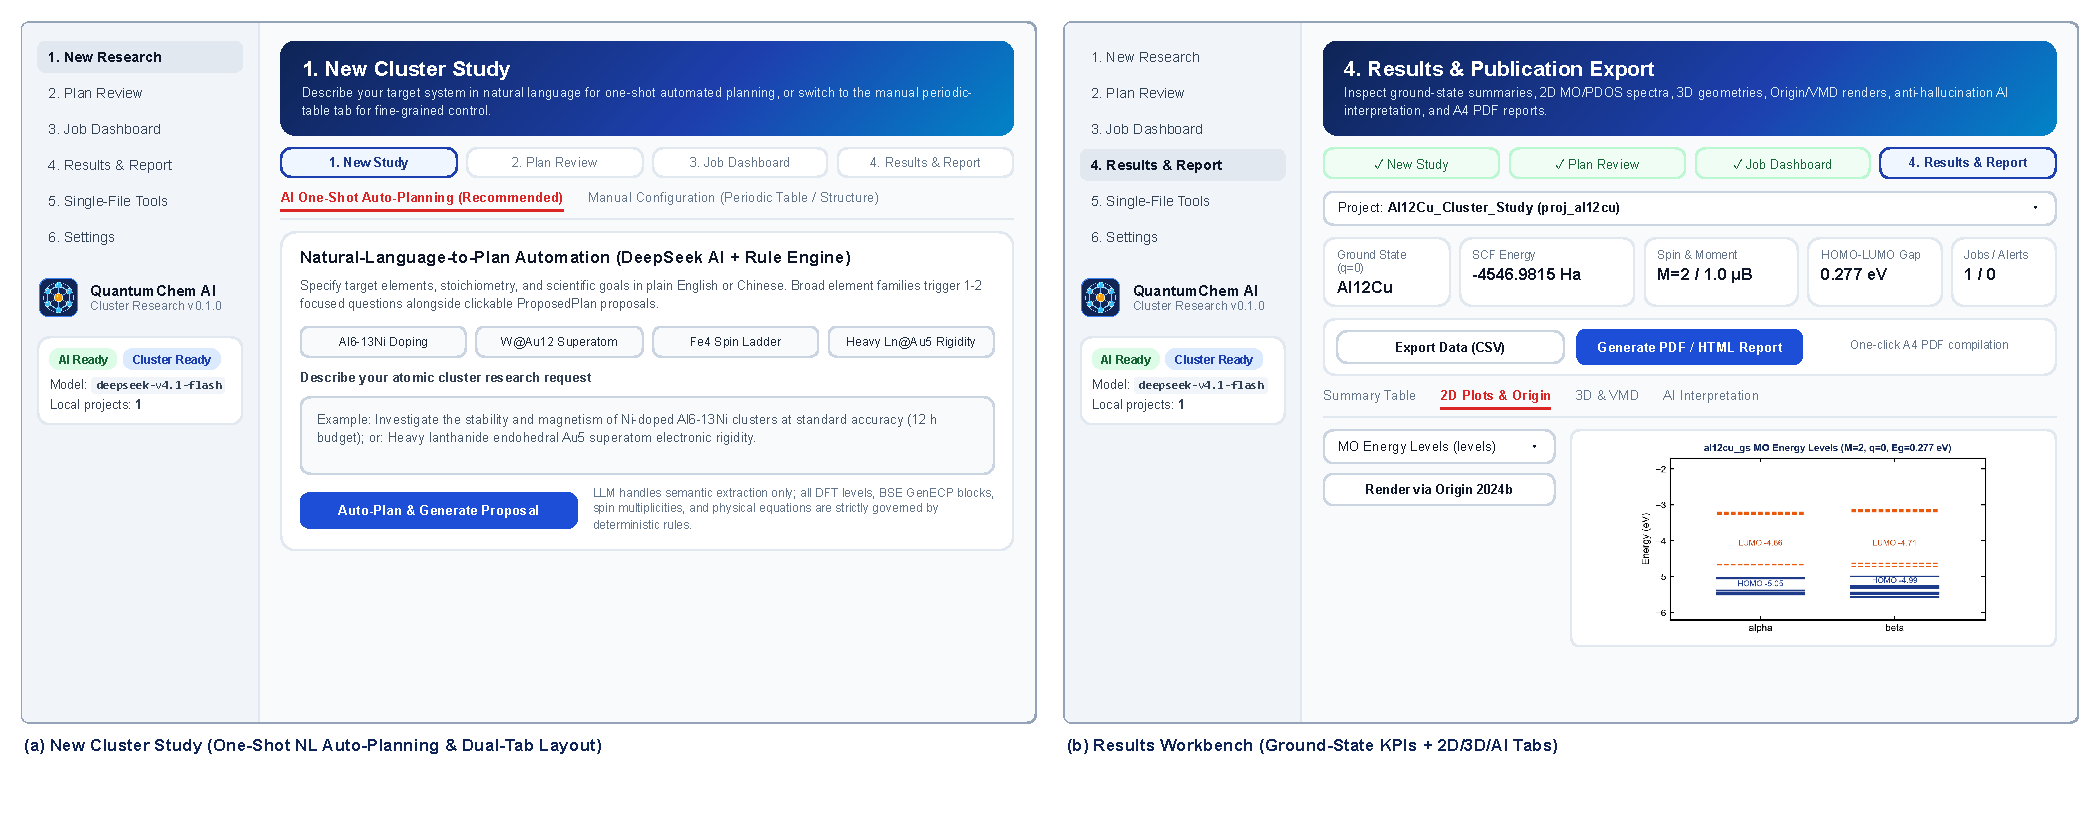
\includegraphics[width=\textwidth]{figures/fig7_web_workbench.pdf}
  \caption{QuantumChem AI interactive web workbench: (a) study setup view supporting natural-language and periodic-table input; (b) results view displaying ground-state summary metrics for $\mathrm{Al_{12}Cu}$, CSV/PDF export controls, and 2D MO/PDOS, 3D geometry, and guarded AI analysis tabs.}
  \label{fig:ui}
\end{figure}

\section{Conclusions}

This work has presented QuantumChem AI, an open-source, rule-governed platform unifying deterministic cluster physics, invariant geometric deduplication, shared-HPC resilience, Multiwfn/Origin/VMD publication workflows, and grounded LLM collaboration. Enforcing the eight-article Design Constitution (C1--C8) via AST static verification, \texttt{build\_plan()} validation, and unit-conversion-aware numerical grounding eliminates element-specific hardcoding and ungrounded AI outputs while maintaining 100.0\% (50/50 Chinese and 50/50 English) natural-language planning accuracy. Across 10 reference Gaussian 16 benchmarks, $\mathrm{Al_{12}Cu}$ wavefunction spectroscopy, and an autonomous 9-project, 230-job (1,399.78 CPU core-hours, 100\% convergence) production study of $\mathrm{Ln@Au_5}$ ($\mathrm{Ln} = \mathrm{Gd\text{--}Lu}$), QuantumChem AI delivers both fault-tolerant automation and clear physical insight into trivalent $8\mathrm{e}^-$ superatom rigidity, localized $4f$ spin decoupling, and divalent $\mathrm{Yb^{2+}}$ electronic transitions.

\section*{Data and Software Availability}

The complete source code of QuantumChem AI is openly distributed under the MIT License (\texttt{LICENSE}) at \url{https://github.com/QIANCHANGKING/quantumchem-ai} and permanently archived on Zenodo under DOI \texttt{10.5281/zenodo.24501860}. The platform targets Python 3.12 (dependency-locked via \texttt{pyproject.toml} and \texttt{uv.lock}) and operates on Windows 10/11 (desktop UI, Origin, VMD, and Chromium PDF generation) and Linux x86\_64 (remote HPC worker execution). All 115 offline unit, AST constitutional-gate, reference benchmark regression, and Playwright E2E tests execute without external HPC access or API credentials.

External computational and visualization software orchestrated by QuantumChem AI are independently obtainable from their providers:
\begin{itemize}
  \item \textbf{Gaussian 16 (Rev.\ C.02):} Commercial license via Gaussian, Inc.\ (\url{https://gaussian.com}).
  \item \textbf{Multiwfn 3.8(dev):} Freely available for academic use (\url{http://sobereva.com/multiwfn/}).
  \item \textbf{Origin 2024b:} Commercial license on Windows via OriginLab Corp.\ (\url{https://www.originlab.com}).
  \item \textbf{VMD:} Freely available for academic use via the Theoretical and Computational Biophysics Group, UIUC (\url{https://www.ks.uiuc.edu/Research/vmd/}).
  \item \textbf{ABCluster and GFN2-xTB (\texttt{tblite}):} Available from their respective academic/open-source distributions for global search and semiempirical screening.
\end{itemize}
All reference benchmark logs (\texttt{tests/data/golden/}), Multiwfn outputs (\texttt{tests/data/multiwfn/al12cu/}), $\mathrm{Ln@Au_5}$ production datasets (\texttt{paper/data/ln\_au5\_summary.json} and \texttt{results/ln\_au5\_study/}), and bilingual 50+50 instruction suites (\texttt{tests/llm\_eval/instructions.yaml} and \texttt{instructions\_en.yaml}) are included in the repository and Supporting Information.

\begin{suppinfo}
Supporting Information contains: (S1) offline installation and 115+ test reproduction guide; (S2) complete YAML rule-engine specification tables; (S3) full 10-benchmark and 19-isomer $\mathrm{Ln@Au_5}$ ($\mathrm{Gd\text{--}Lu}$) quantitative tables, 7 server-side \texttt{custodian} recovery traces, and Cartesian coordinates (\AA); and (S4) complete 50+50 bilingual natural-language instruction evaluation breakdown.
\end{suppinfo}

\begin{acknowledgement}
The author acknowledges local Linux compute cluster resources for the multi-day $\mathrm{Ln@Au_5}$ production campaign. ORCID: \url{https://orcid.org/0009-0005-2464-3814}.
\end{acknowledgement}

\section*{Notes}
The author declares no competing financial interest.

\bibliography{references}

\begin{tocentry}
  \centering
  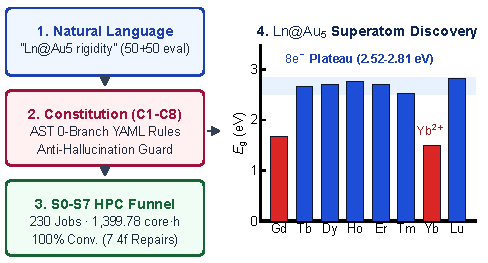
\includegraphics[width=3.20in]{figures/TOC_graphic.pdf}
\end{tocentry}

\end{document}
